\documentclass[main.tex]{subfiles}

%\externalcitedocument{bibfile}

\begin{document}

\section{IceCube Upgrade}

Introduce physics goals of IceCube upgrade, show some plots that compare old v new event displays. 

Upgrade is shown in Figure~\ref{fig:upgrade_layout}

\begin{figure}
    \centering
    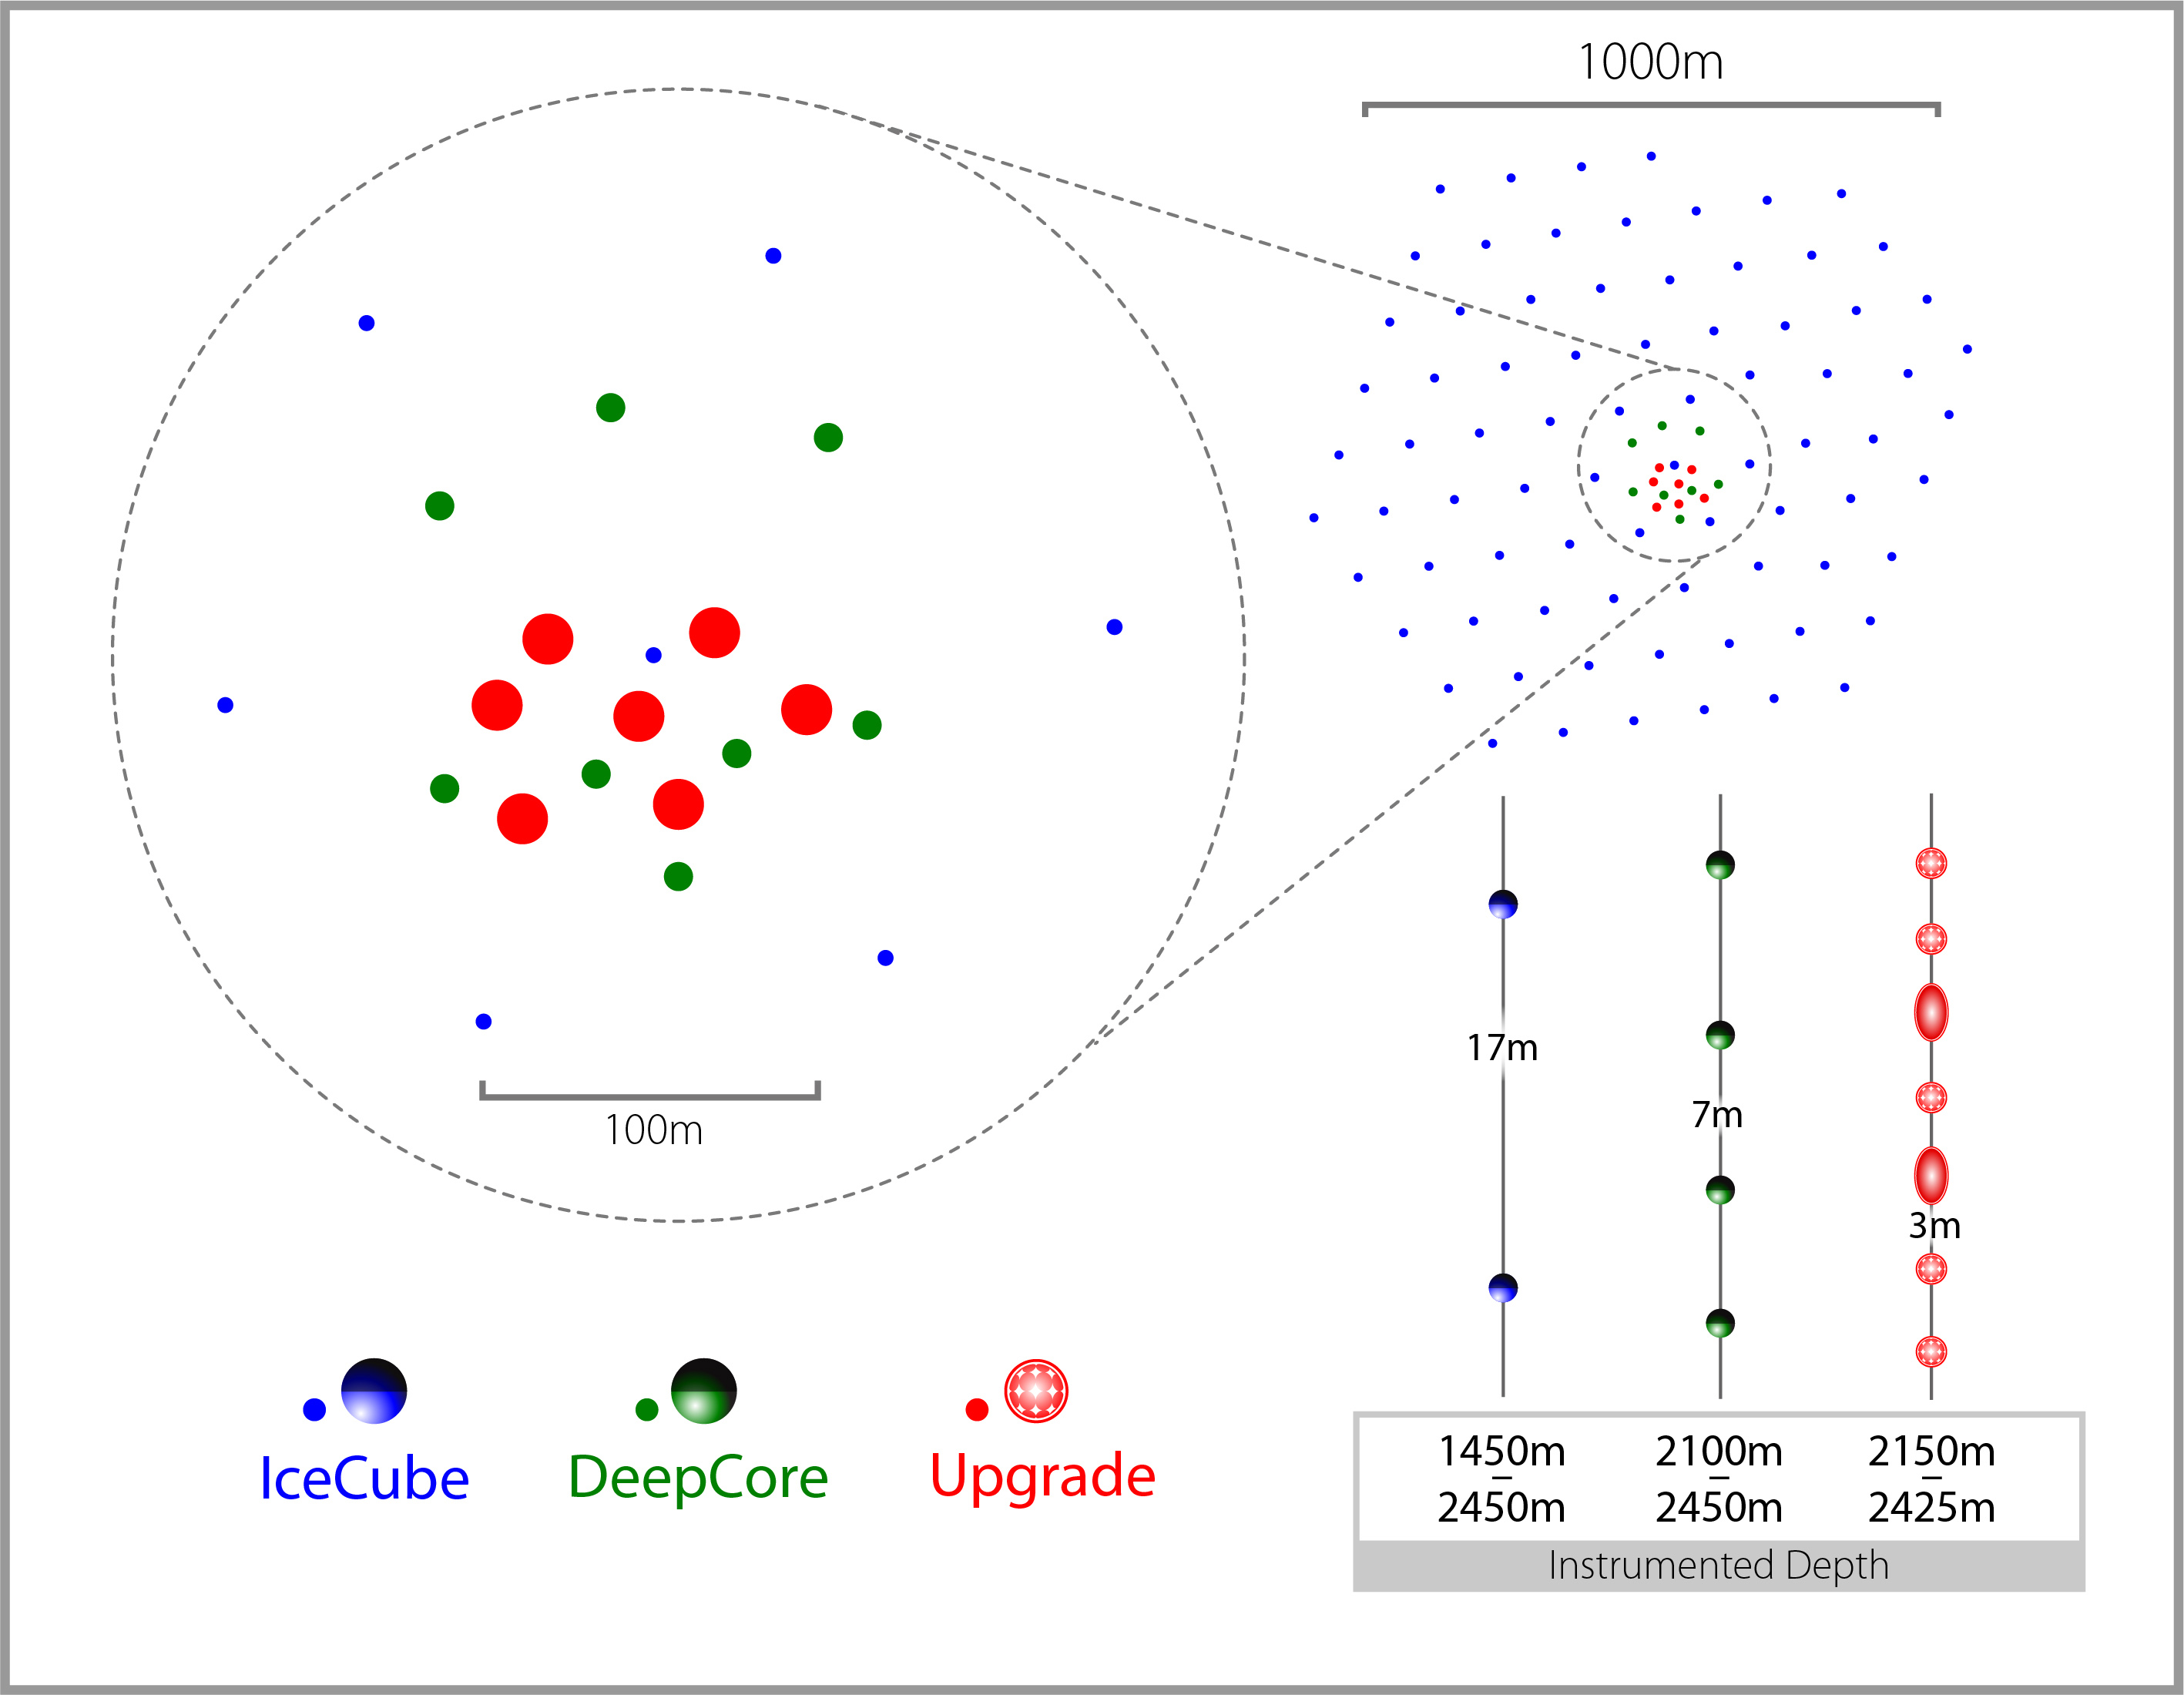
\includegraphics[width=\linewidth]{figures/ICUpgradeLayout_V4b.jpg}
    \caption{A top-down view of the planned installation locations of IceCube Upgrade strings relative to existing IceCube and DeepCore strings.}
    \label{fig:upgrade_layout}
\end{figure}

\section{IceCube D-Eggs}

The ``\textbf{D}ual optical sensors in an \textbf{E}llipsoid \textbf{G}lass for \textbf{G}en2,'' or D-Egg, is a new module designed for future extensions of IceCube. 
A diagram of a D-Egg is shown in Figure~\ref{fig:degg}
In particular, it is one of the planned optical modules to be deployed at the IceCube Neutrino Observatory as part of IceCube Upgrade, witha planned deployment in the 2025-2026 South Pole season.
The D-Eggs have been designed with an elongated egg-like shape and narrow cross section to maximize its photon-sensitive area while maintaining a slim shape to reduce the time needed for deployment-hole drilling in the Antarctic ice to depths of up to 2,700 meters. 
Two PMTs are used per D-Egg: one each facing upwards and downwards. 

\begin{figure}
    \centering
    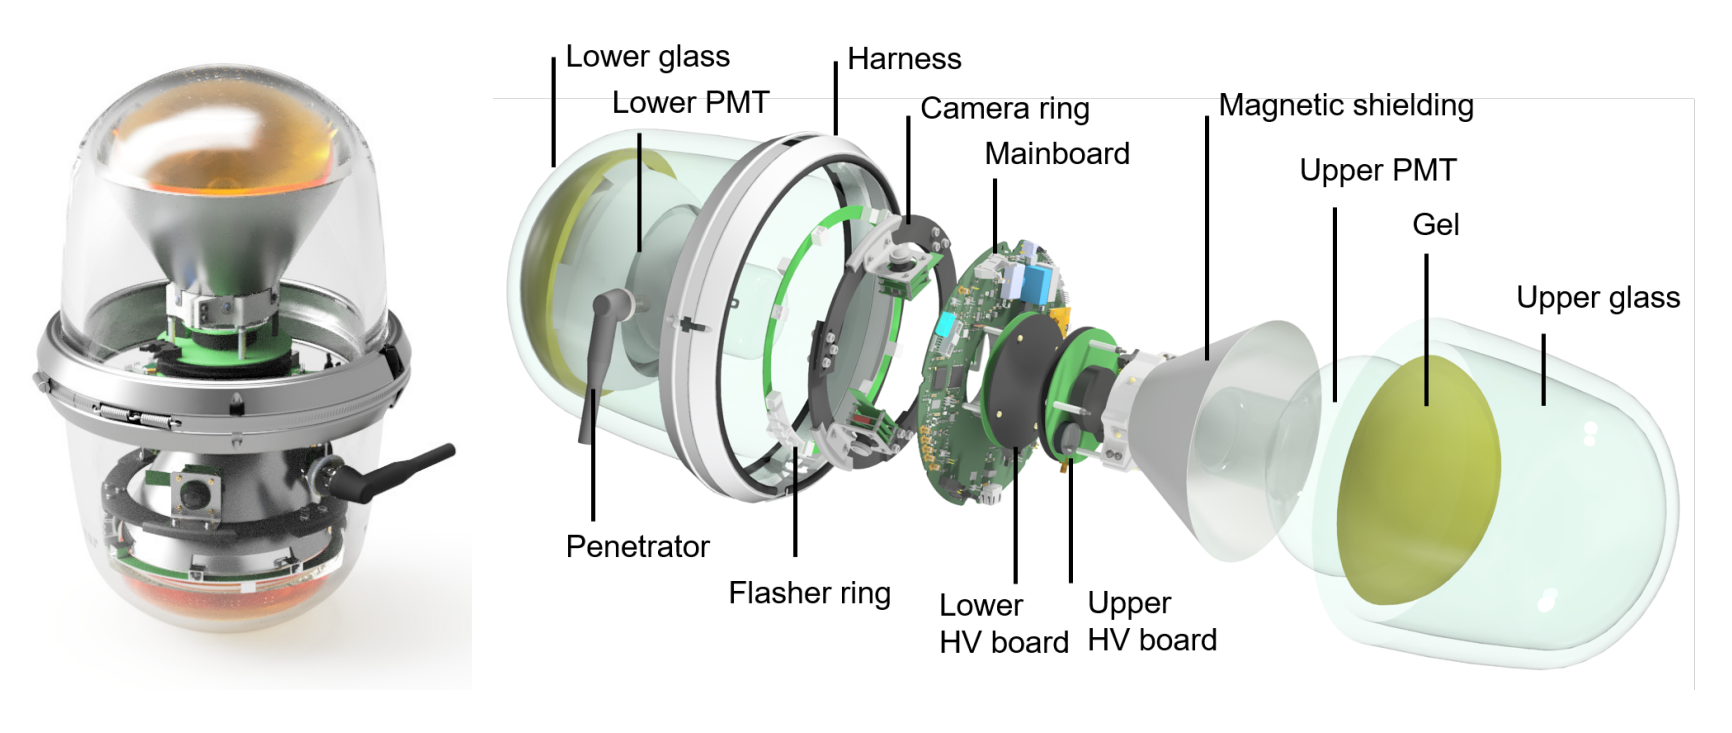
\includegraphics[width=\linewidth]{figures/degg.png}
    \caption{(left) A D-Egg with the harness around its equator, which is used to hold the device during deployment, and its sealed UV-transparent glass housing. (right) An exploded figuring showing the D-Egg internal structure, including: the mainboard, three cameras, twelve LED flashers, two PMTs, optical coupling silicone gel, and the emagnetic shielding.}\label{fig:degg}
\end{figure}

\section{Final Acceptance Testing of D-Eggs}

For the Final Acceptance Testing (FAT), D-Eggs are tested in batches of fifteen D-Eggs plus one reference D-Egg. 
They are lifted into a freezer, capable of reaching temperatures as low as negative sixty degrees Celcius, and placed into light-sealed boxes in order to isolate individual D-Eggs from one another. 
Optical fibers and insulated cables are routed into the freezer to provide communications, power, and light sources to each D-Egg. 

IceBoot sessions are then established with the D-Eggs and we begin taking measurements. 
Measurements are taken on a consistent basis as the freezer is brought to negative forty degrees Celcius, then up to negative twenty again, back down to negative forty, and then returned to room temperature (approximately twenty degrees Celcius). 

\begin{figure}
    \centering
    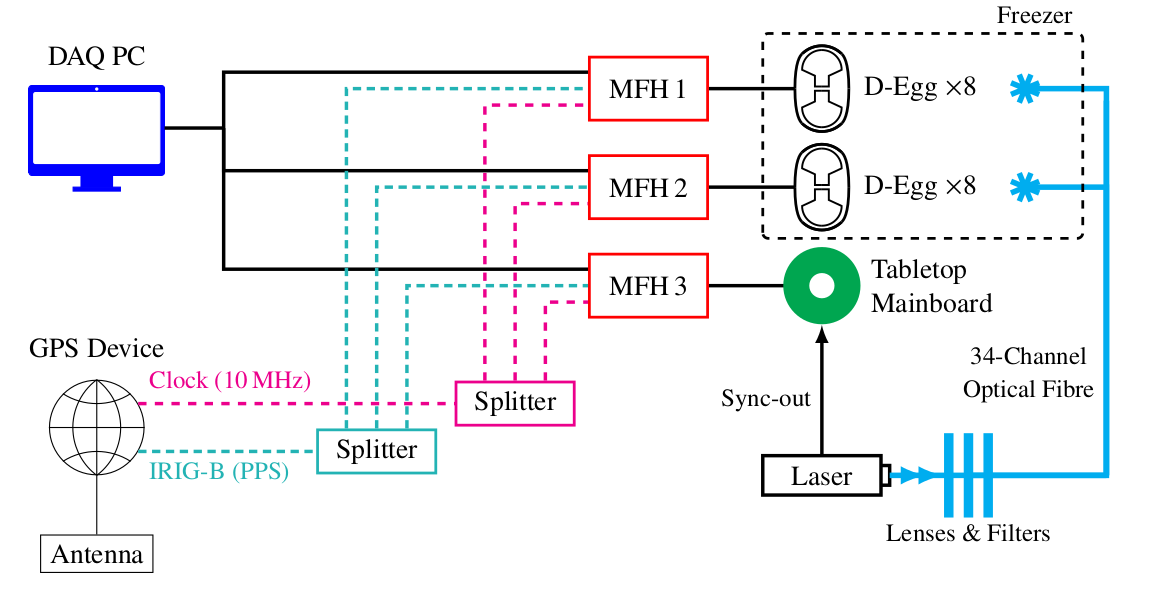
\includegraphics[width=\linewidth]{figures/fat_layout.png}
    \caption{A schematic layout of the FAT layout. }
    \label{fig:fatscheme}
\end{figure}

The block-diagram FAT facility is shown in Figure~\ref{fig:fatscheme}. 
A dedicated data aquisition (DAQ) computer, or DAQ PC, is used to communicate with D-Eggs via two Mini FieldHubs (MFHs); these are simplified versions of the hardware used on-site at the South Pole to communicate with in-ice DOMs. 
A third MFH is used to synchronize timing between a pulsed laser source and the other two MFHs. 
The light source used is a Hamamatsu PLP-10 C10196 with a 400 nm picosecond laser diode head M10306.
Two programmable filter wheels with six distinct neutral density filters are used to attenuate the laser light by discrete amounts. 
The laser light is carried through optical fiber to expose both the top and bottom PMTs of each D-Egg.
This allows for the characterization of the gain of each D-Egg PMT at light levels ranging from low-occupancy SPE to more than 200 SPE levels. 

A 10 MHz clock and the IRIB-B GPS time signals are split and fed into each of the MFHs to synchronize their internal clocks to UTC.
This allows for conversion of the internal D-Egg timestamps to UTC using the standard IceCube Reciprocal Active Pulsing (RAPCal) method~\cite{ABBASI2009294}.


\subsection{Quick Monitoring}

\subsection{Detailed Monitoring}

As the temperature in the freezer is moving to its new target temperature, gain scans are regularly performed on the D-Eggs. 
The D-Egg PMTs have been independently measured to have an SPE pulse full-width half-maximum of approximately 14 nanoseconds and an amplitude of approximately 12 mV. 
Mainboard electronics on the D-Eggs broaden these pulses to an approximate amplitude of 6mV and FWHM of 20ns. 
As such, a trigger threshold of 2.0mV is typically used.

To calculate the gain, a charge distribution is first constructed from the read-out SPE waveforms by integrating from ten bins before the peak to fifteen bins after it.
A Gaussian is then fitted to the charge histogram, whose peak corresponds to the PMT voltage at a given set high-toltage. An example SPE waveform and charge distribution is shown in Figure~FIG.
This procedure is repeated at varrying high voltages until the calculated gain is within $\pm 2\%$ of $10^{7}$.
A typical high voltage found is around 1500V. 

\subsection{Analyses}

Once the measurements are taken, data are transfered from the local DAQ PC to the grappa server system in Chiba. Several analyses are then performed. 
First, a fit is performed to check for a linear relationship between gain and the set PMT high-voltage.  
The dark-rate of the PMTs is then 

\end{document}